
\documentclass[../main.tex]{subfiles}

\begin{document}

Results of the query generation experiment are shown in Table \ref{tbl_results}. Overall, LeafAI matched 212 of 427 (49\%) total enrolled patients across 8 clinical trials compared to 180 (42\%) found by queries of the human programmer. The mean per-trial percent of patients matched was 43.5\% for LeafAI and 27.2\% for the human programmer. LeafAI had a greater number of patients deemed eligible across trials, for a total of 27,225 eligible compared to 14,587 found by the human programmer. 

\begin{table}[h!]
    \small
    \centering
    
\documentclass[../main.tex]{subfiles}

\begin{document}

Results of our evalution are shown in Table \ref{tbl_results}.

\begin{table}[h!]
    \small
    \centering
    
\documentclass[../main.tex]{subfiles}

\begin{document}

Results of our evalution are shown in Table \ref{tbl_results}.

\begin{table}[h!]
    \small
    \centering
    
\documentclass[../main.tex]{subfiles}

\begin{document}

Results of our evalution are shown in Table \ref{tbl_results}.

\begin{table}[h!]
    \small
    \centering
    \input{tables/results}
    \caption{}
    \label{tbl_results}
\end{table} 

\begin{figure}[h!]
  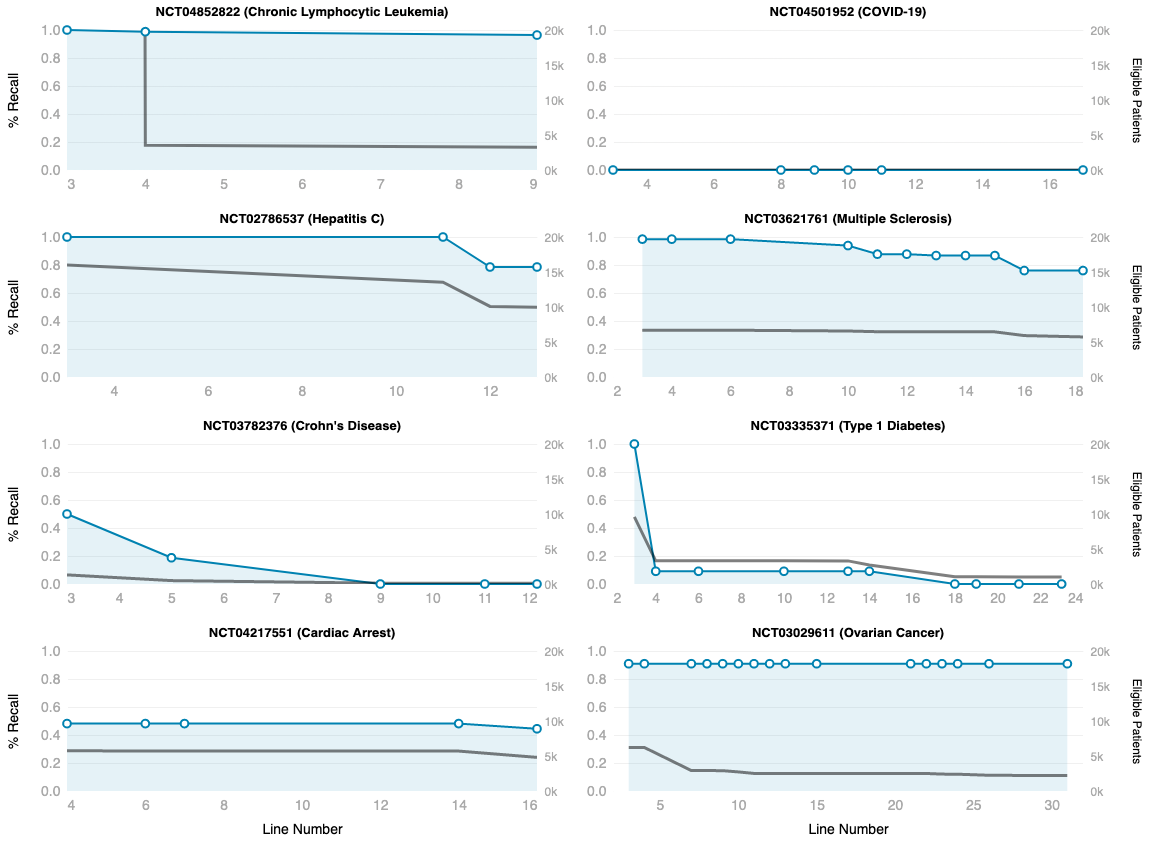
\includegraphics[scale=0.42]{figures/leafai_detail_results_longitudinal.png}  
\caption{}
\label{fig_leafai_results_longitudinal}
\end{figure}

\begin{table}[h!]
    \small
    \centering
    \input{tables/results_leafai_detail}
    \caption{}
    \label{tbl_results_leafai_detail}
\end{table} 


\end{document}
    \caption{}
    \label{tbl_results}
\end{table} 

\begin{figure}[h!]
  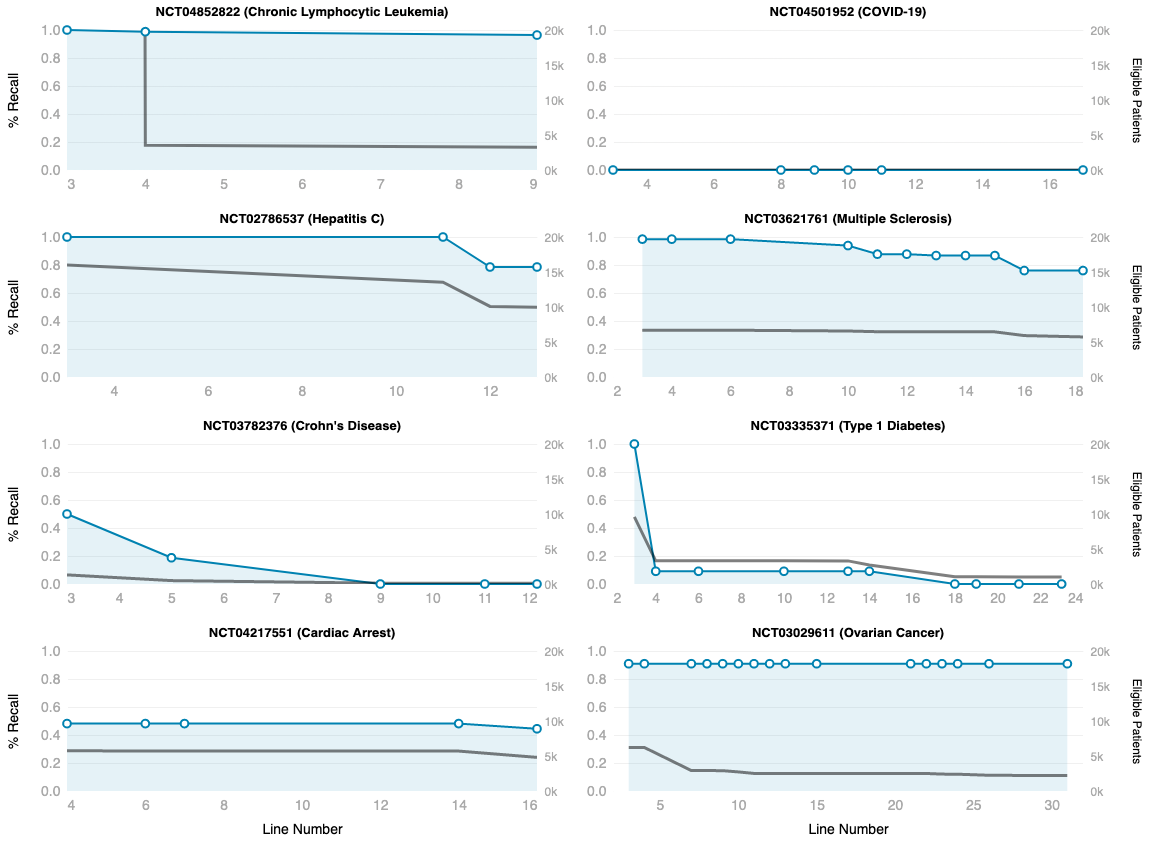
\includegraphics[scale=0.42]{figures/leafai_detail_results_longitudinal.png}  
\caption{}
\label{fig_leafai_results_longitudinal}
\end{figure}

\begin{table}[h!]
    \small
    \centering
    \def\arraystretch{1.4}
\begin{tabular}{l c c c c}
    \textbf{Condition} & \textbf{\# Criteria} & \textbf{Skipped - \newline No Patients} & \textbf{Skipped - \newline Not Computable} & \textbf{Fully Executed} \\
    \toprule
    Cl Lymphoma        & 4  & 0 (0\%)    & 0 (0\%)    & 4  (100\%)  \\
    Hepatitis C        & 8  & 0 (0\%)    & 4 (50\%)   & 4  (50\%)   \\
    Crohn's Disease    & 9  & 0 (0\%)    & 4 (44.4\%) & 5  (55.5\%) \\
    Cardiac Arrest     & 12 & 0 (0\%)    & 8 (66.6\%) & 4  (33.3\%) \\
    COVID-19           & 13 & 0 (0\%)    & 6 (46.1\%) & 7  (53.8\%) \\
    Multiple Sclerosis & 14 & 1 (7.1\%)  & 3 (21.4\%) & 10 (71.4\%) \\
    Type 1 Diabetes    & 18 & 2 (11.1\%) & 8 (44.4)   & 8  (44.4\%) \\
    Ovarian Cancer     & 25 & 2 (8\%)    & 9 (36\%)   & 14 (56\%)   \\
    \bottomrule
    \textbf{Total} & 103 & 5 (4.8\%) & 42 (40.7\%) & 61 (59.3\%)
\end{tabular}
    \caption{}
    \label{tbl_results_leafai_detail}
\end{table} 


\end{document}
    \caption{}
    \label{tbl_results}
\end{table} 

\begin{figure}[h!]
  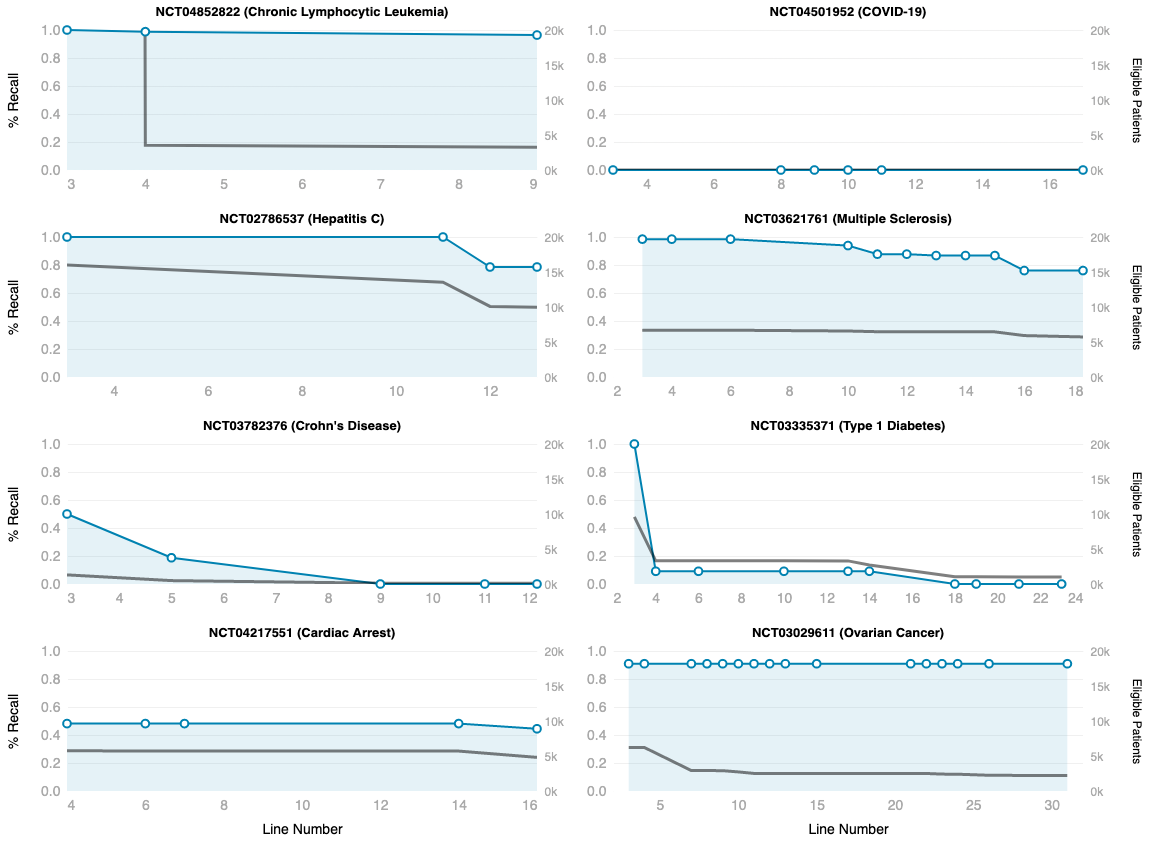
\includegraphics[scale=0.42]{figures/leafai_detail_results_longitudinal.png}  
\caption{}
\label{fig_leafai_results_longitudinal}
\end{figure}

\begin{table}[h!]
    \small
    \centering
    \def\arraystretch{1.4}
\begin{tabular}{l c c c c}
    \textbf{Condition} & \textbf{\# Criteria} & \textbf{Skipped - \newline No Patients} & \textbf{Skipped - \newline Not Computable} & \textbf{Fully Executed} \\
    \toprule
    Cl Lymphoma        & 4  & 0 (0\%)    & 0 (0\%)    & 4  (100\%)  \\
    Hepatitis C        & 8  & 0 (0\%)    & 4 (50\%)   & 4  (50\%)   \\
    Crohn's Disease    & 9  & 0 (0\%)    & 4 (44.4\%) & 5  (55.5\%) \\
    Cardiac Arrest     & 12 & 0 (0\%)    & 8 (66.6\%) & 4  (33.3\%) \\
    COVID-19           & 13 & 0 (0\%)    & 6 (46.1\%) & 7  (53.8\%) \\
    Multiple Sclerosis & 14 & 1 (7.1\%)  & 3 (21.4\%) & 10 (71.4\%) \\
    Type 1 Diabetes    & 18 & 2 (11.1\%) & 8 (44.4)   & 8  (44.4\%) \\
    Ovarian Cancer     & 25 & 2 (8\%)    & 9 (36\%)   & 14 (56\%)   \\
    \bottomrule
    \textbf{Total} & 103 & 5 (4.8\%) & 42 (40.7\%) & 61 (59.3\%)
\end{tabular}
    \caption{}
    \label{tbl_results_leafai_detail}
\end{table} 


\end{document}
    \caption{Statistics for each clinical trial evaluated by the LeafAI query engine and human programmer. The number of enrolled and matched patients were determined by cross-matching enrollments listed within our EHR. The \textit{Time} column indicates the number of hours the human programmer spent developing queries for each trial.}
    \label{tbl_results}
\end{table} 

Table \ref{tbl_results_leafai_detail} shows the number of criteria which were skipped by LeafAI. Of the 103 total criteria across all 8 studies, LeafAI executed queries for 61 (59.3\%) and skipped 5 (4.8\%) as it found no patients and 42 (40.7\%) because no computable concepts were found. 

\begin{table}[h!]
    \small
    \centering
    \def\arraystretch{1.4}
\begin{tabular}{l c c c c c}
    \textbf{Condition} & \textbf{\# Criteria} & \textbf{\# No Patients} & \textbf{\# Not Computable} & \textbf{\# Fully Executed} \\
    \toprule
    Cl Lymphoma        & 4  & 0 (0\%)    & 0 (0\%)    & 4  (100\%)  \\
    Hepatitis C        & 8  & 0 (0\%)    & 4 (50\%)   & 4  (50\%)   \\
    Crohn's Disease    & 9  & 0 (0\%)    & 4 (44.4\%) & 5  (55.5\%) \\
    Cardiac Arrest     & 12 & 0 (0\%)    & 8 (66.6\%) & 4  (33.3\%) \\
    COVID-19           & 13 & 0 (0\%)    & 6 (46.1\%) & 7  (53.8\%) \\
    Multiple Sclerosis & 14 & 1 (7.1\%)  & 3 (21.4\%) & 10 (71.4\%) \\
    Type 1 Diabetes    & 18 & 2 (11.1\%) & 8 (44.4)   & 8  (44.4\%) \\
    Ovarian Cancer     & 25 & 2 (8\%)    & 9 (36\%)   & 14 (56\%)   \\
    \bottomrule
    \textbf{Total}     & 103 & 5 (4.8\%) & 42 (40.7\%) & 61 (59.3\%)
\end{tabular}
    \caption{The LeafAI query engine's handling of eligibility criteria for each trial. The column \textit{No Patients} indicates the count of criteria which would, if executed, cause no patients to be eligible. The column \textit{Not Computable} indicates the count of criteria which LeafAI could not generate a query for, for various reasons. Both of these types of criteria were ignored by the system.}
    \label{tbl_results_leafai_detail}
\end{table} 

Figure \ref{fig_leafai_results_analysis} shows longitudinal results from four trials with commentary indicating differences in query strategy by LeafAI and the human programmer. 

\begin{figure}[H]
  \begin{center}
    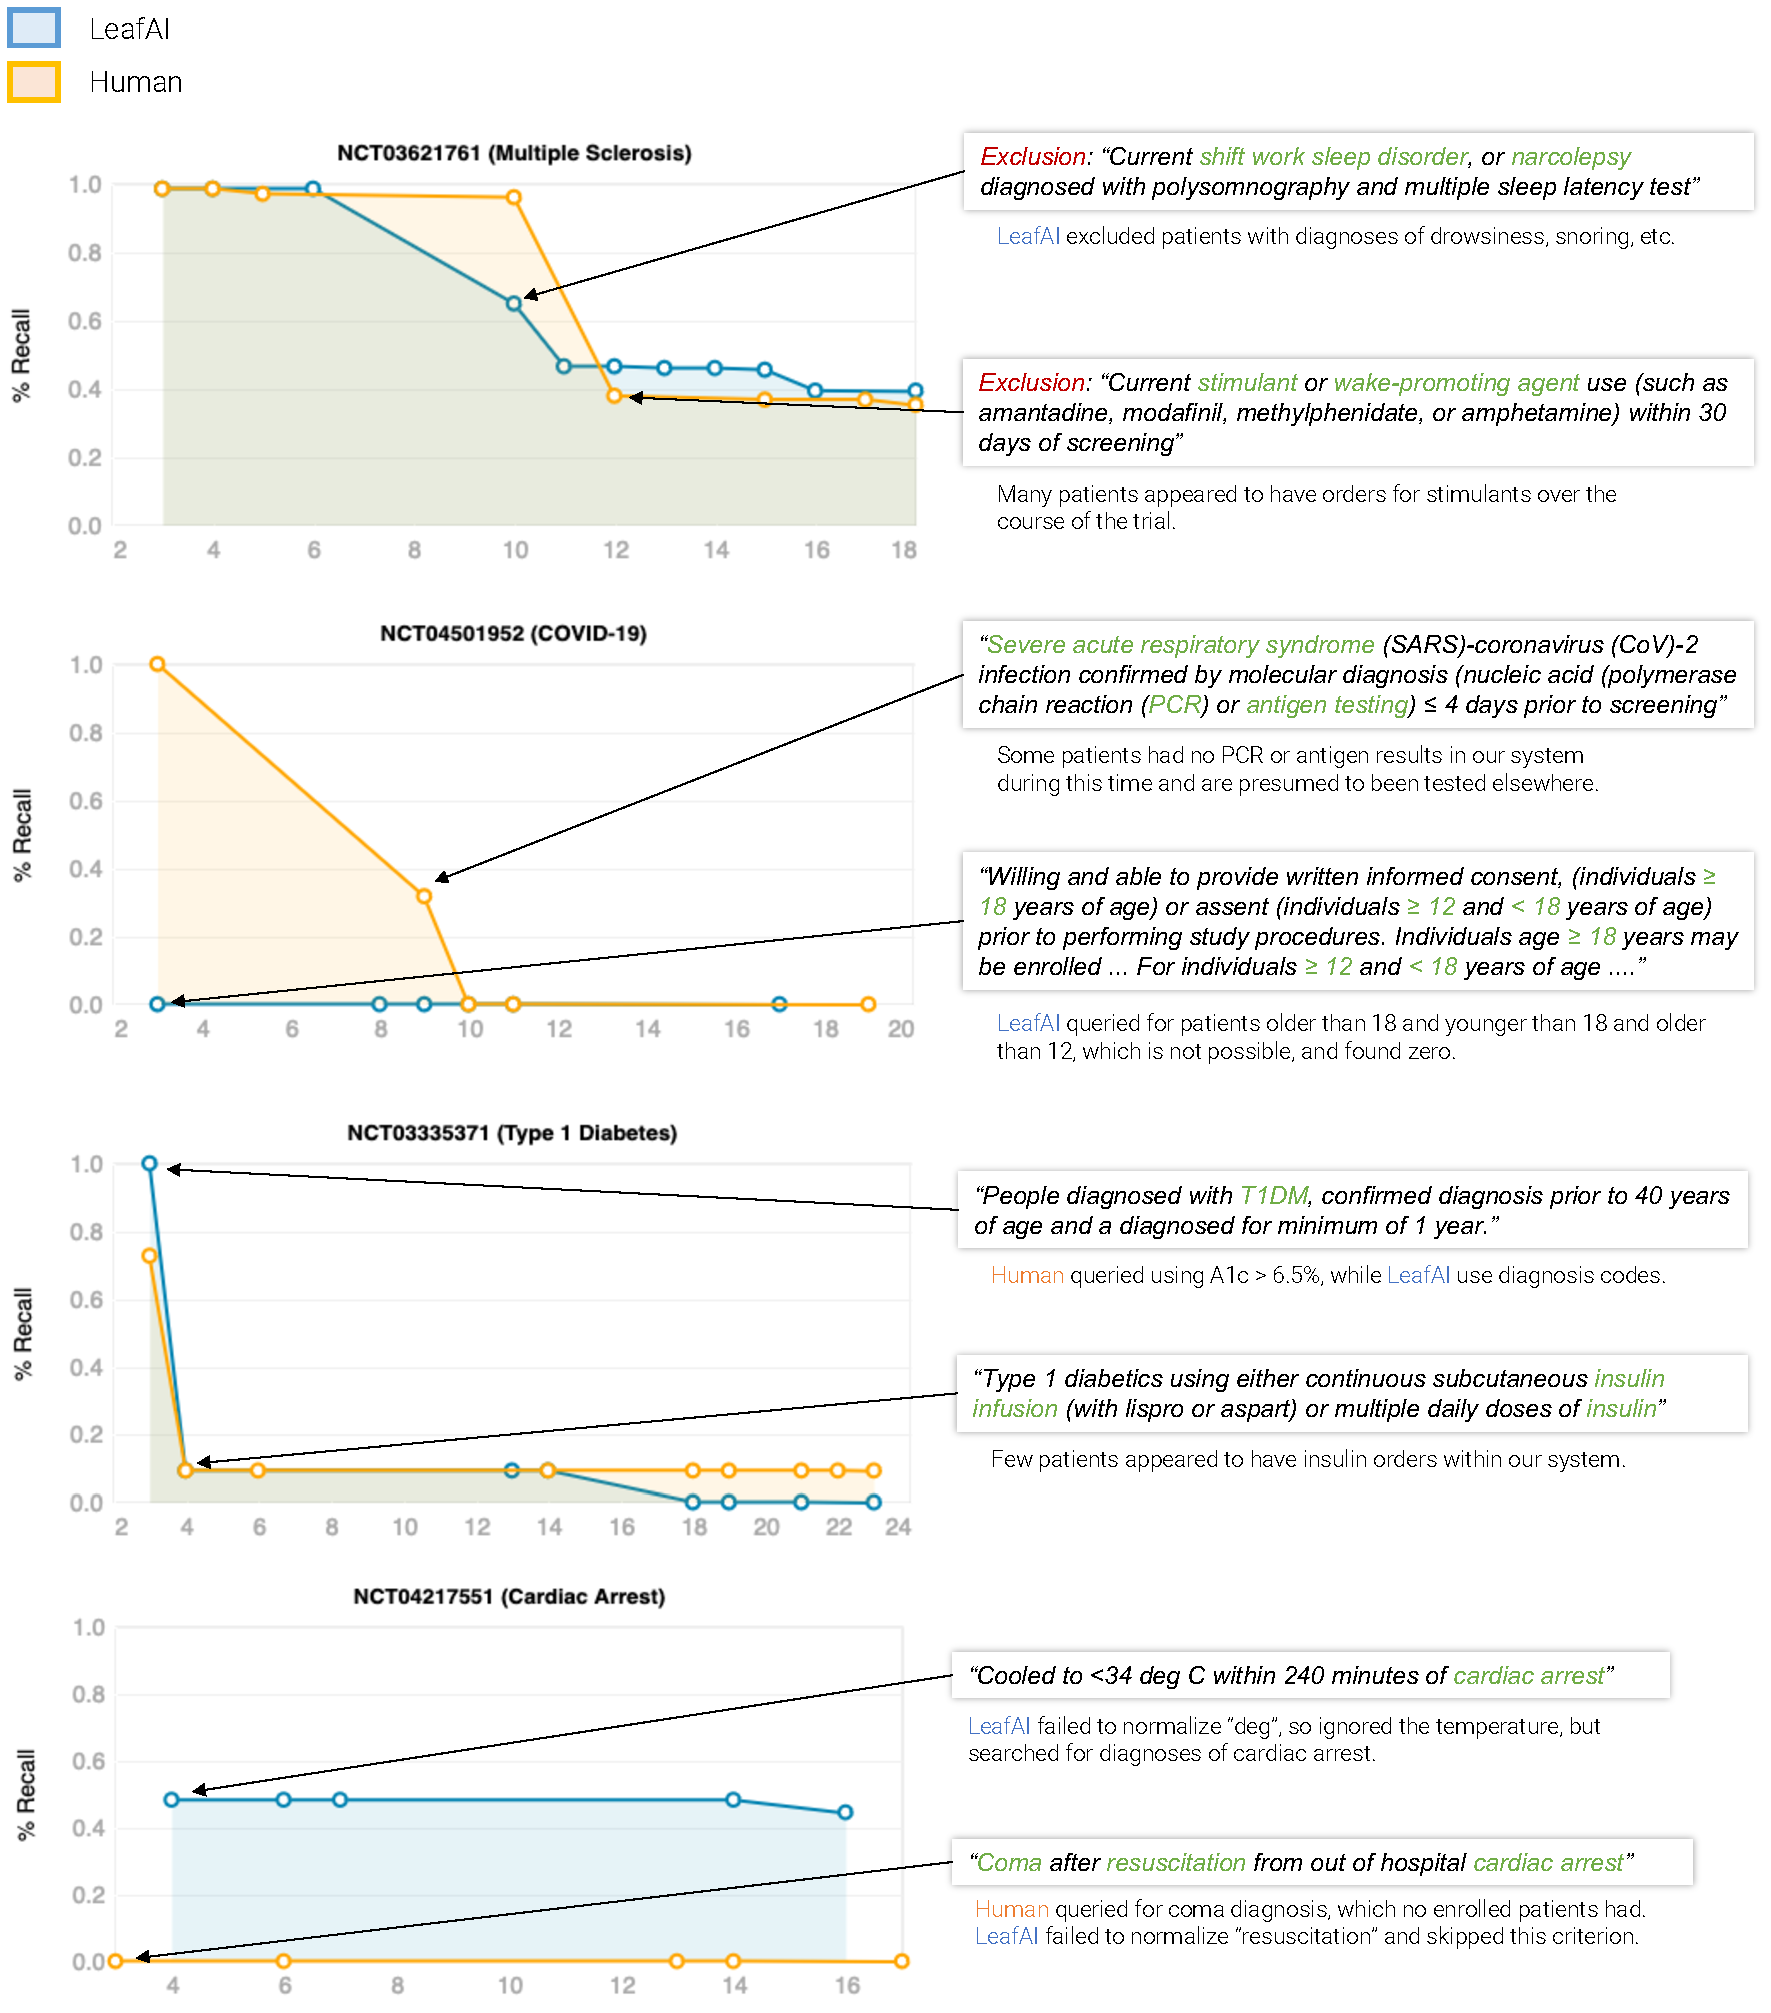
\includegraphics[scale=0.51]{figures/leafai_paper2_analysis0.pdf}  
  \end{center}
  \caption{Longitudinal results listing patients found at each step in the query process for four representative trials. The blue line indicates \% recall for LeafAI and orange that of the human programmer. The X axis represents the line number within the free-text eligibility criteria. Dots indicate that a query was executed for a given line. On the right, boxes represent the text of a given eligibility criteria, with comments below discussing strategies of LeafAI and the human programmer and findings related to available data.}
  \label{fig_leafai_results_analysis}
\end{figure}

\end{document}